\section{External LEDs and Push Buttons}

\subsection{Parts List}


\begin{enumerate}[itemsep=-5pt]
  \item Laptop
  \item CPX + USB Cable
  \item 2 Alligator clips
  \item Push Button
  \item Breadboard
  \item LED (Light Emitting Diode) (x3 in case you fry some)
  \item Resistor (300 to 1000 Ohms)
\end{enumerate}

\subsection{Learning Objectives}

\begin{enumerate}[itemsep=-5pt]
\item The VOUT and 3.3V pin are always "ON" even when code is not
  running on the CPX. So long as your CPX is plugged in via USB or a
  Lipo Battery
\item LED are Light Emitting {\bf Diodes} which means current only flows in one direction
\item LEDs need resistors in series otherwise they will get too hot and burn up
\item Breadboard pinout diagrams
\item Analog pins can be controlled by simply using the digitalio module
\item LEDs can be hooked up to analog pins and set to blink by changing the board pin
\end{enumerate}

In this project we’re going to use the same blink code as before but
modify it to blink an external LED. The purpose of this lab is to
familiarize yourself with the pins on the CPX and create a simple
circuit using the 5V pin on the CPX and one of the Analog pins. Your
laptop has a battery with something between 10 to 20V. There are DC to
DC converters in your laptop that provide 5V to your USB ports. These
USB ports can be used to power your CPX as you have done in the past
few labs.

If you purchased the optional
\href{https://www.adafruit.com/product/3287}{battery pack} you can
also power the CPX using 3 AA batteries. These batteries nominally
have 1.5 V but fully 
charged it's actually something like 1.8 V. So 1.8 times 3 is 5.4V
which is enough to power the CPX. If you have the battery pack and
some AA batteries, give it a try. If you still have the blink code
from the last project on board you’ll see the D13 LED blink as
before. You won’t be able to see the serial print() output as before
but that code will be running which is why D13 is blinking. {\bf I have
noticed that some of the battery packs have power and ground wires
swapped. If the battery pack doesn’t work it may be because those two
wires are backwards.}

The CPX itself uses 3.3V logic which means when it converts numbers to
binary a 0 (False) represents 0 volts and a 1 (True) represents
3.3V. The CPX has ports that are labeled various things. GND stands
for ground and you need to hook the negative end of your circuit to
this and it also has VOUT which supplies 5V to any circuit you
build. Hook the positive end of your circuit to the VOUT pin. There is
also a port labeled 3.3V and obviously that outputs 3.3V

You’re going to need to use a breadboard so if you’re not familiar
with how breadboards work I would recommend watching this \href{https://www.youtube.com/watch?v=mE33WpRWrXs}{video on how
breadboards work}. Your lab today specifically involves an external
LED. You can read about
\href{https://learn.sparkfun.com/tutorials/light-emitting-diodes-leds/}{LEDs}
more online if you wish. {\bf Remember that the long leg of the LED is 
the positive end and the short leg is the negative end.} The task today
is to wire an LED up to the CPX in the following ways

{\bf Whenever you modify a circuit on the breadboard, always be sure
  to remove power from the CPX. You can damage multiple components if
  you’re not careful.}

\subsection{LED with no Code}

For this part we are going to light up the LED without the use of any
code on the CPX. First, wire up the circuit with the positive end
connected to 5V. This is how my circuit looks. Make sure to use a
resistor between 300 and 1000 Ohms. An LED does not have that much
internal resistance so you need a resistor in series with an LED to
reduce the amount of current flowing through the LED or the entire LED
will fry. If you use a resistor that has too much impedance the LED
just won’t turn on because the voltage/current through the LED will be
below the activation voltage of the circuit. 
\begin{figure}[H]
  \begin{center}
    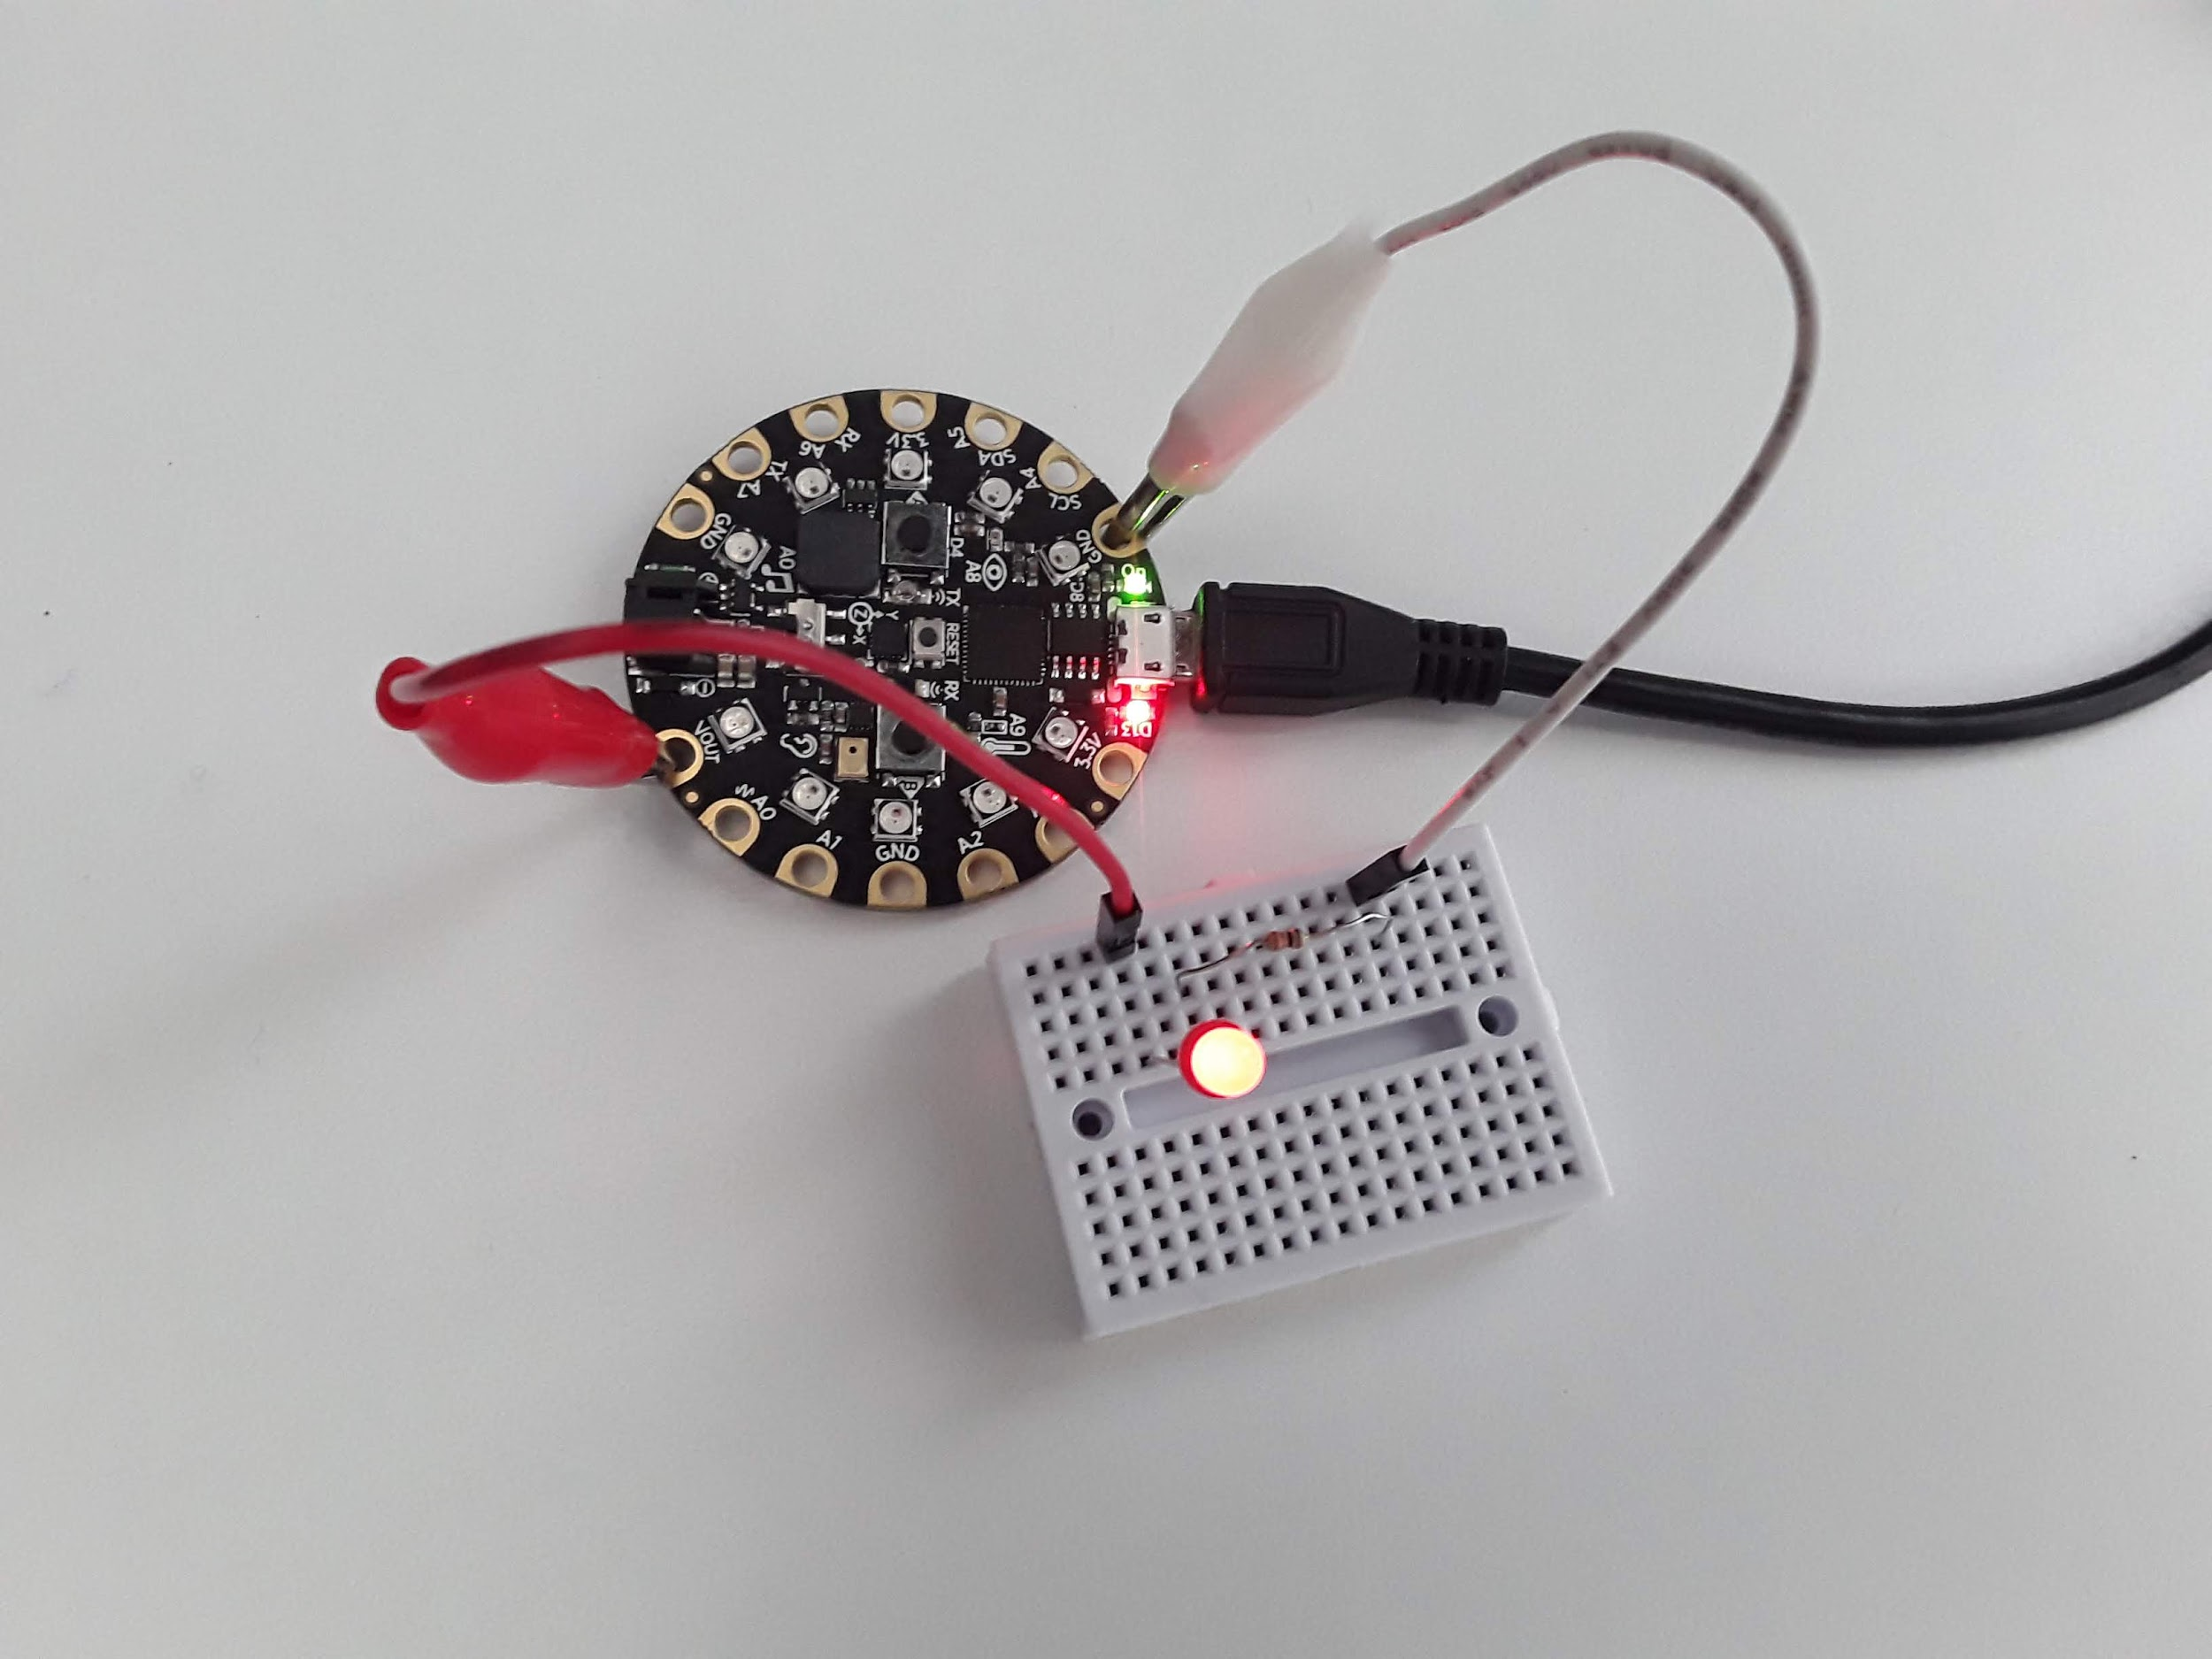
\includegraphics[width=\textwidth]{Figures/LED1.jpeg}
  \end{center}
\end{figure}
Once you have that circuit working, wire up the circuit again with the
3.3V output. Do you notice anything different when you hook up the
circuit with different pins? Here’s my circuit. Do you notice
something different about the intensity of the LED? Why is it
different?
\begin{figure}[H]
  \begin{center}
    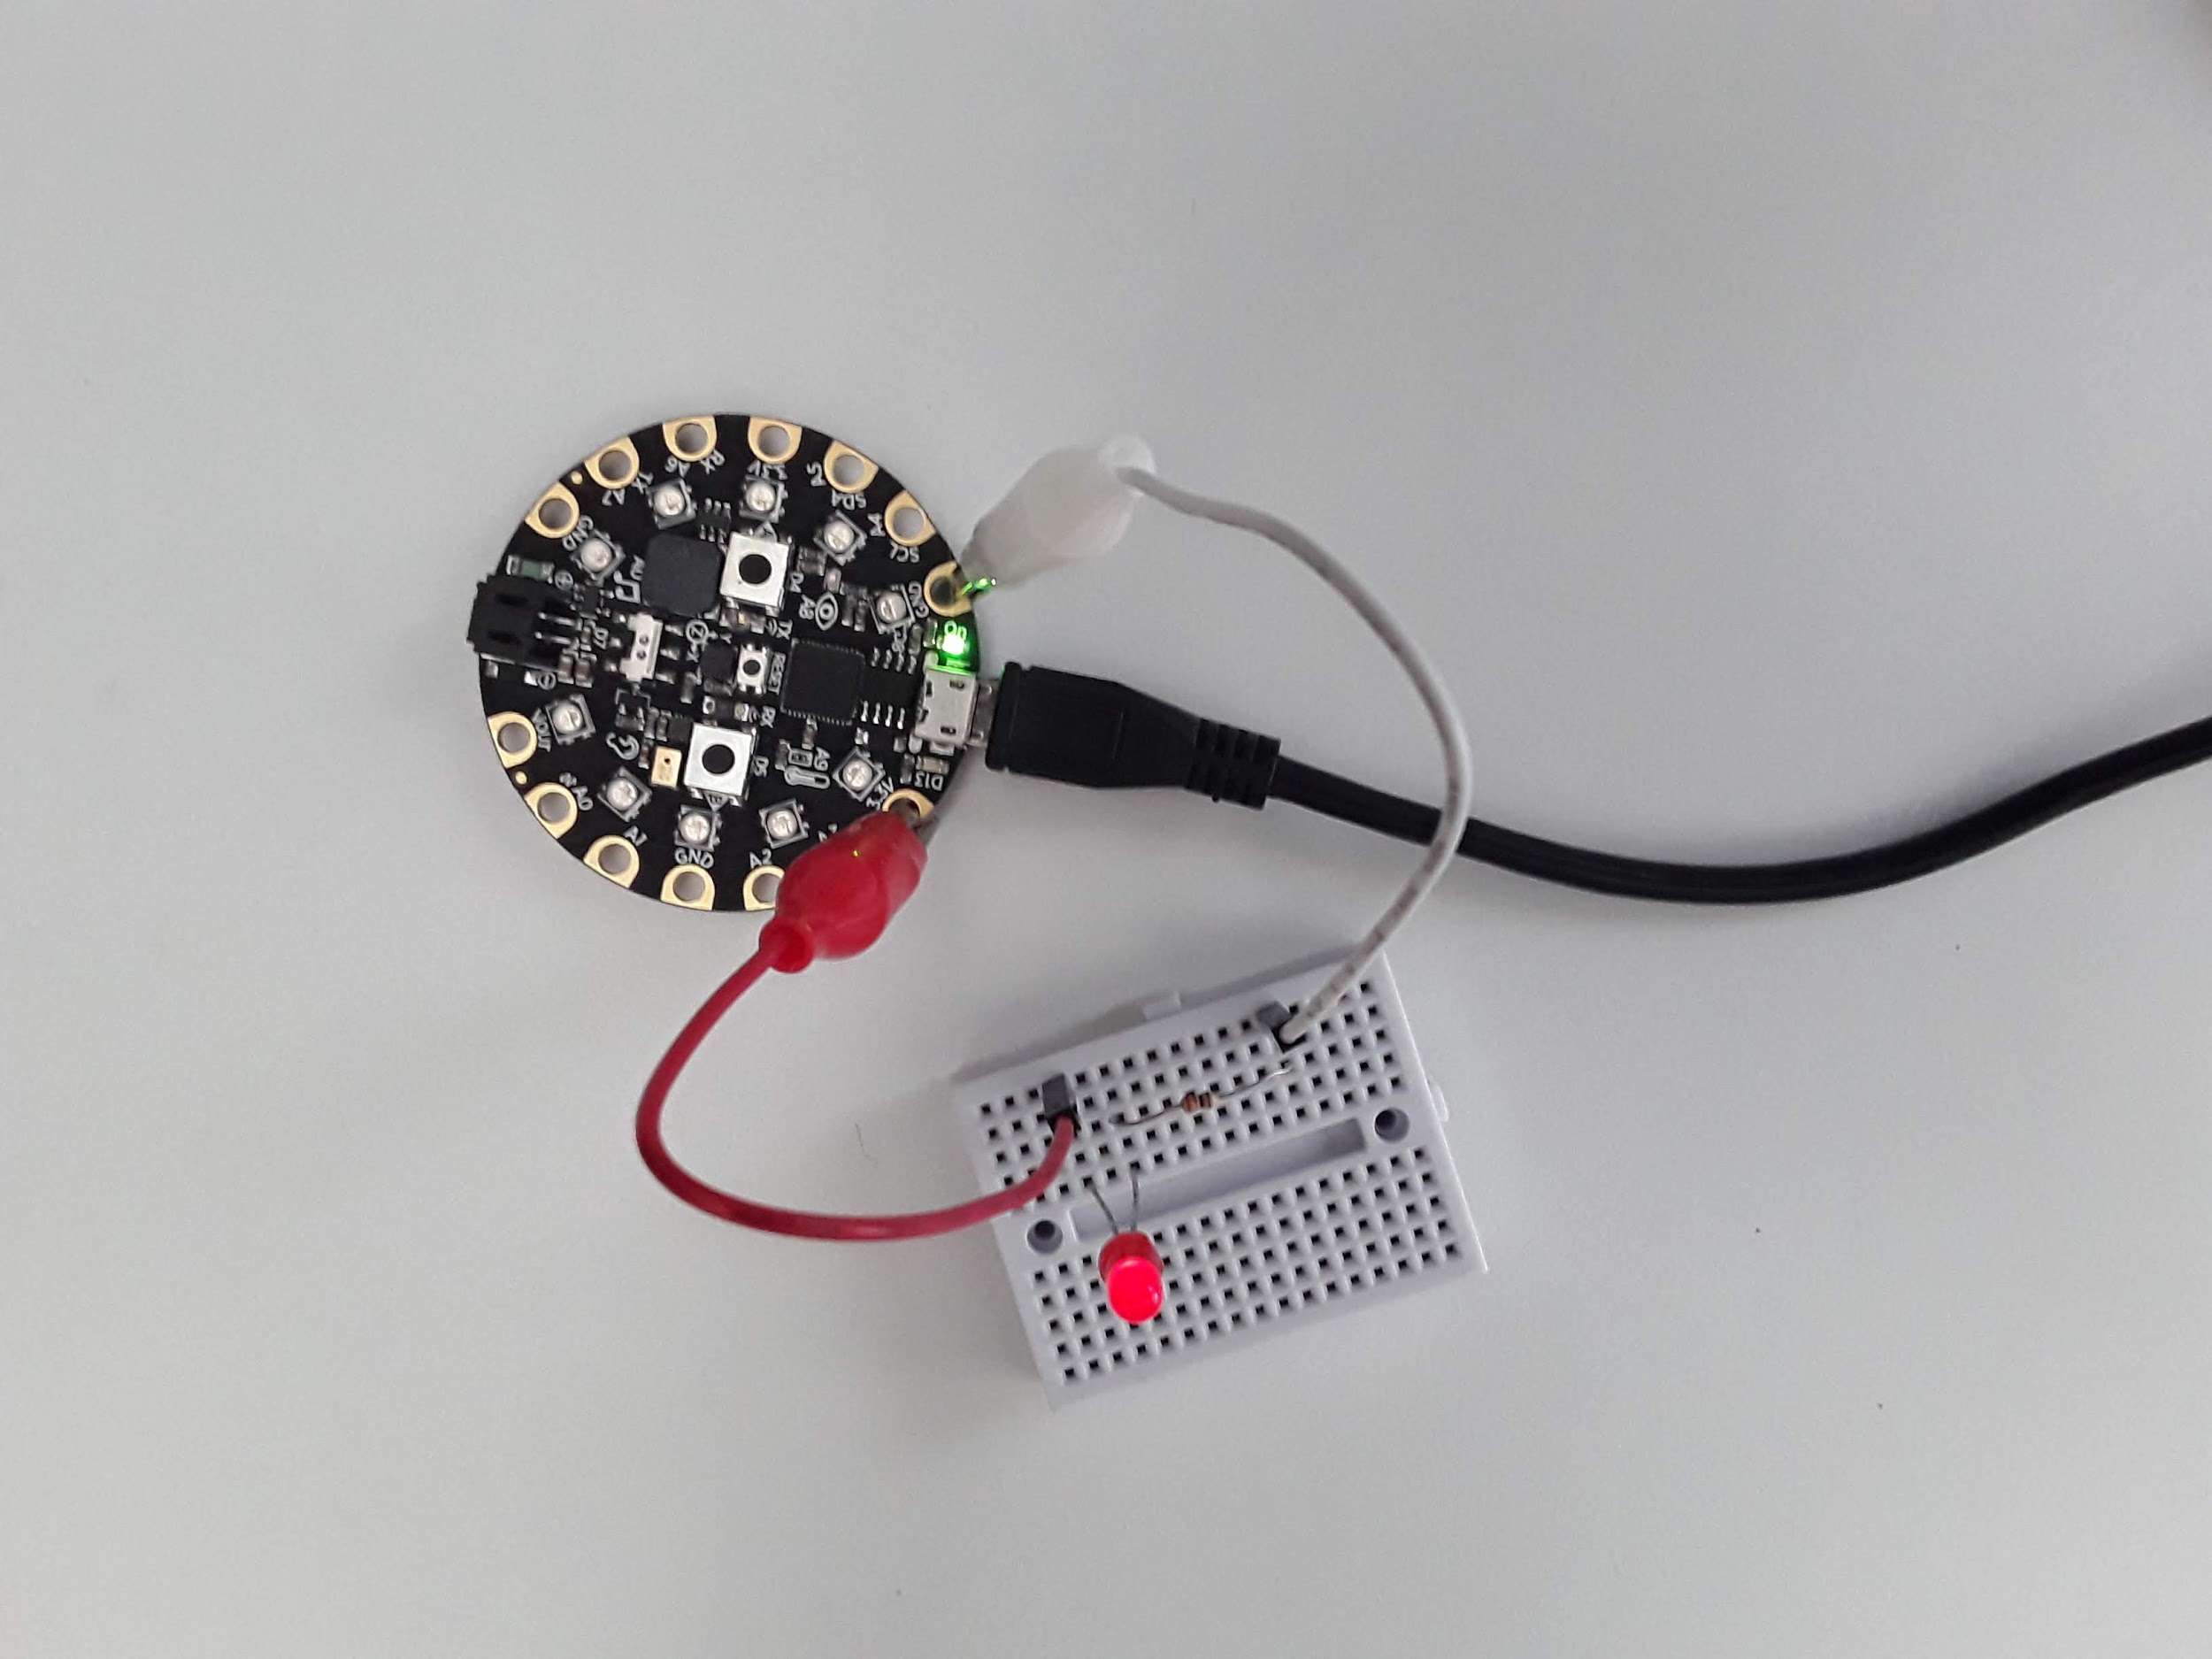
\includegraphics[width=\textwidth]{Figures/LED2.jpeg}
  \end{center}
\end{figure}
\subsection{LED with a push button}

Now that we understand breadboards a bit, we’re now going to manually
blink the LED using a push button placed 
onto the breadboard and have it act like a switch. Therefore, when the
button is pressed, the LED will turn on and when the button is
released the LED will turn off. The button just acts like a wire so
you can plug in the button anywhere in the circuit.
\begin{figure}[H]
  \begin{center}
    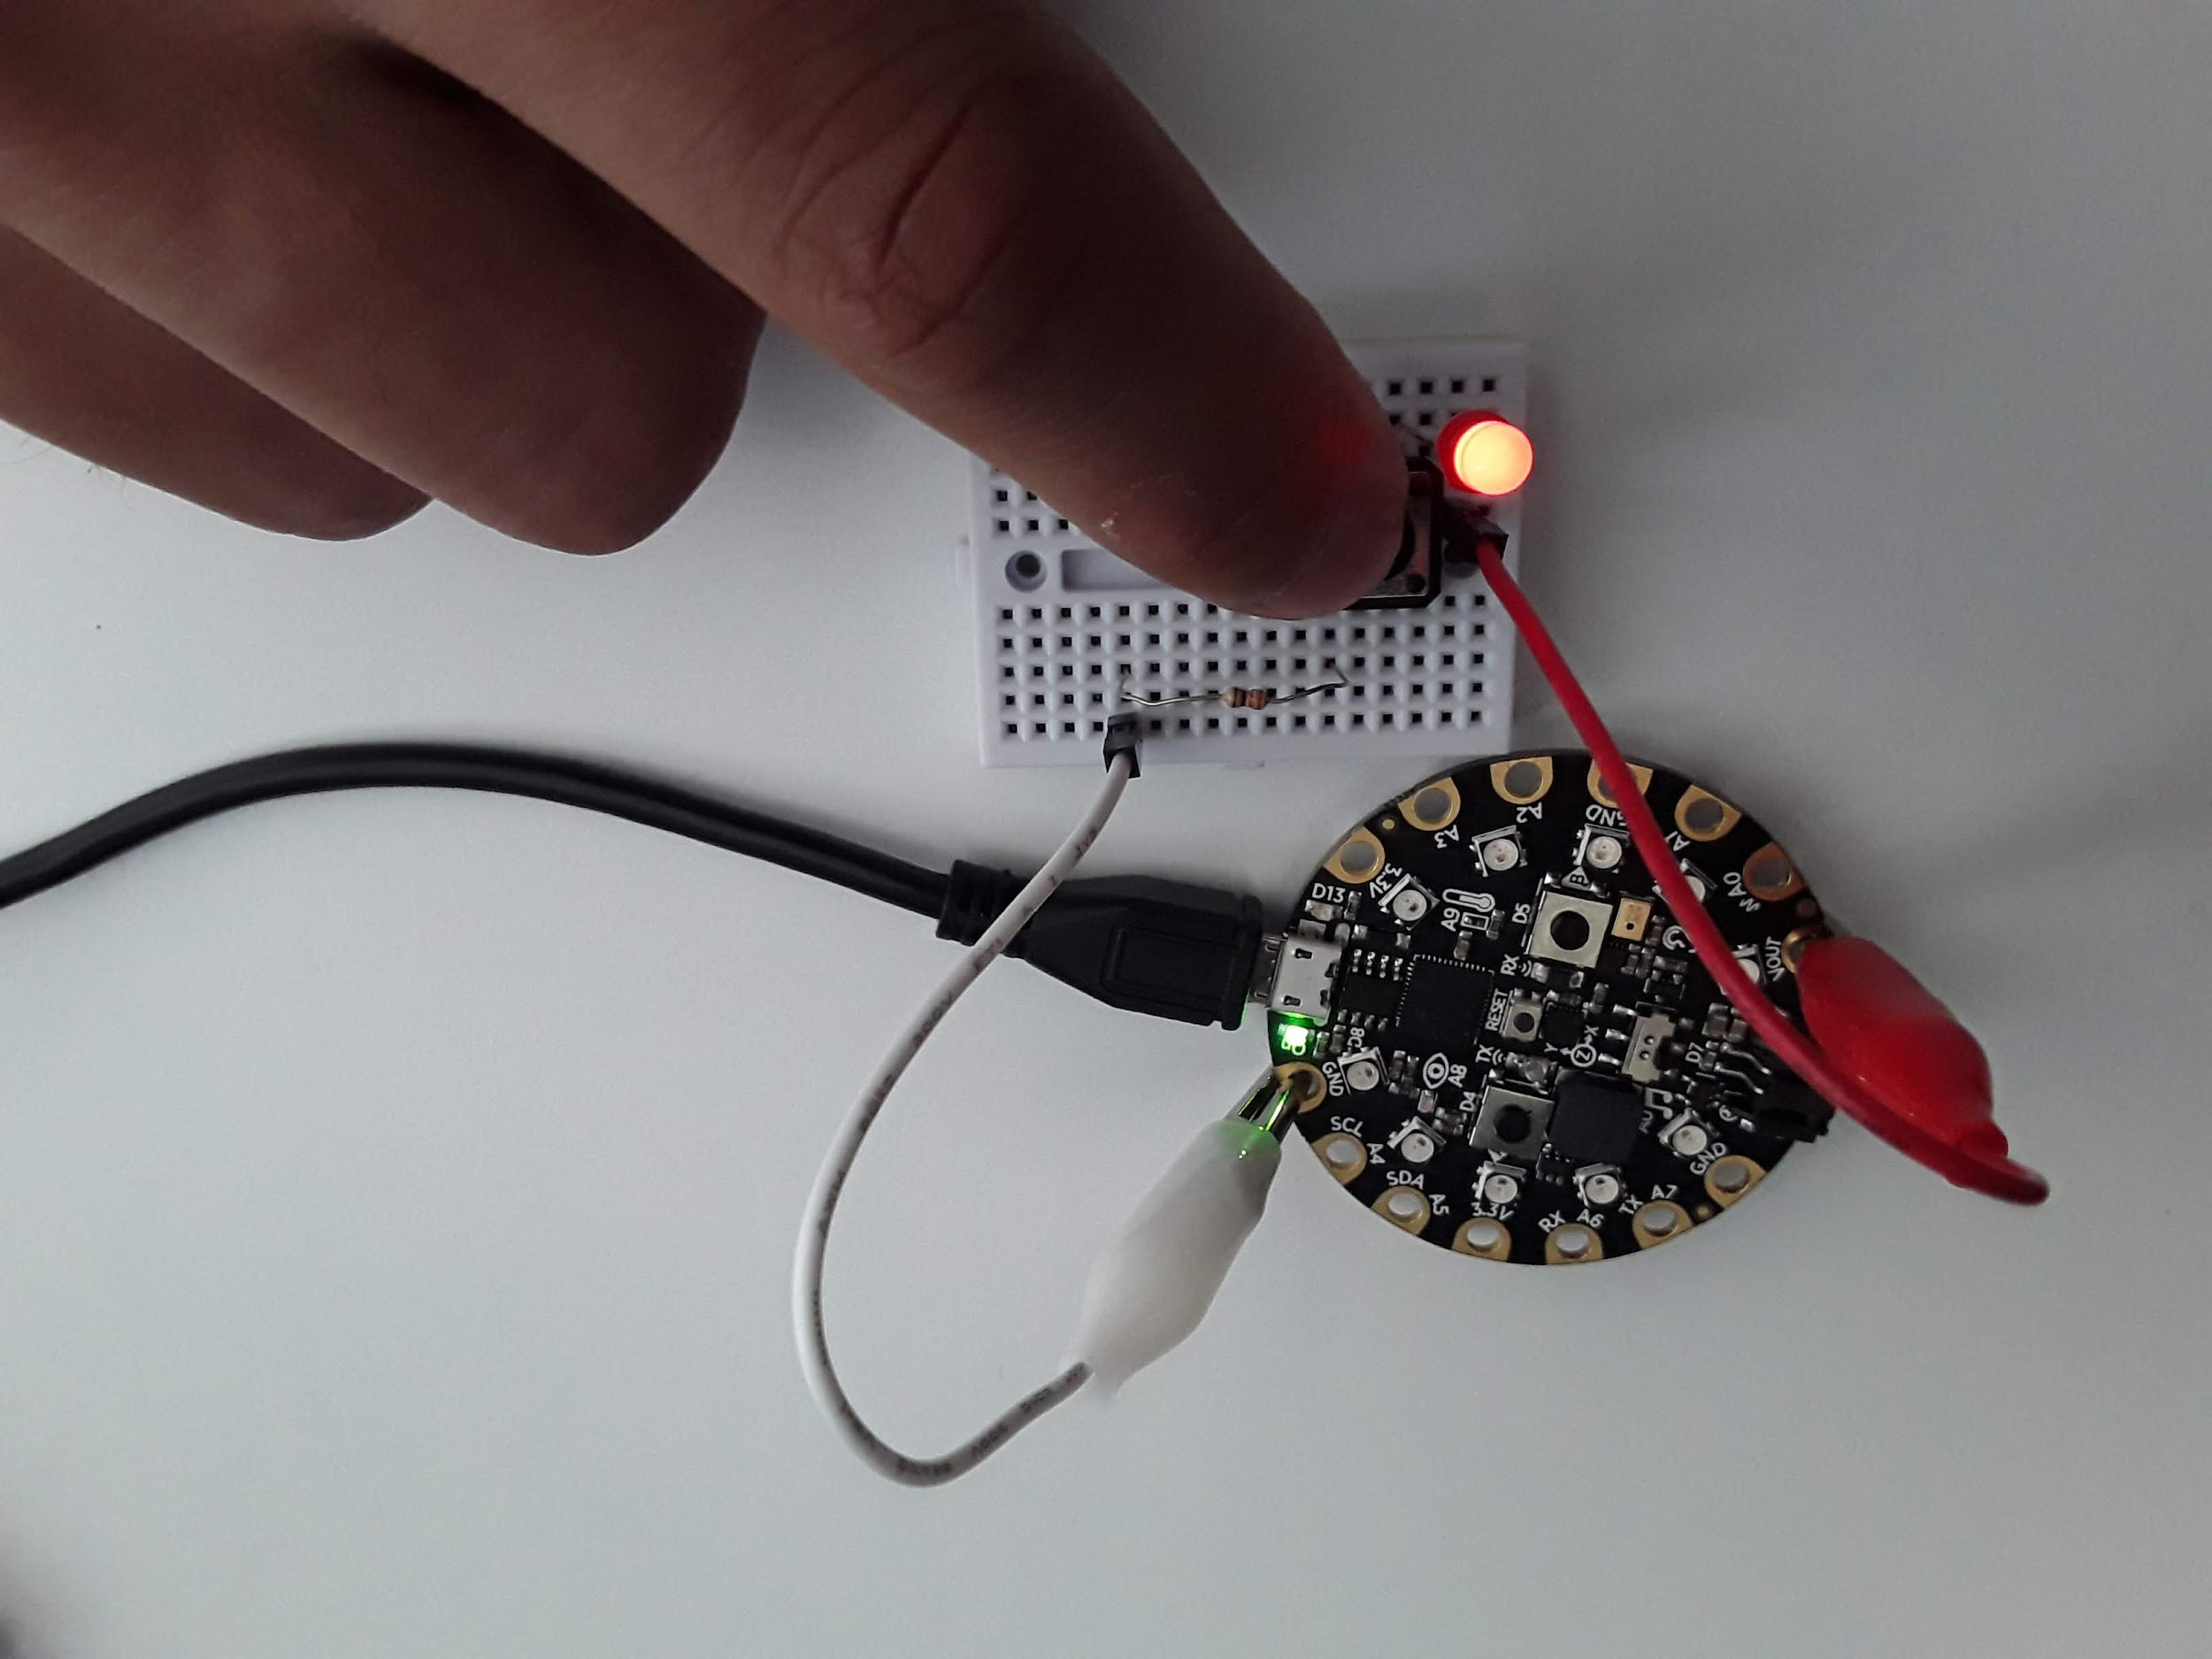
\includegraphics[width=\textwidth]{Figures/LED3.jpeg}
  \end{center}
\end{figure}

\subsection{LED with code}

Next I want you to remove the button from the circuit and wire up the
LED like you had it when the positive end was connected to VOUT or
3.3V. Except this time I want you to hook the positive end of the
circuit to pin A2. Then edit your blink code to blink pin A2. Take
a look at the blink 
code. Right now the code is blinking pin D13. How do you think you
need to change the code to blink pin A2? Here’s what my circuit looks
like for this one. I won’t include code for this one since you just
need to change one line of code.
\begin{figure}[H]
  \begin{center}
    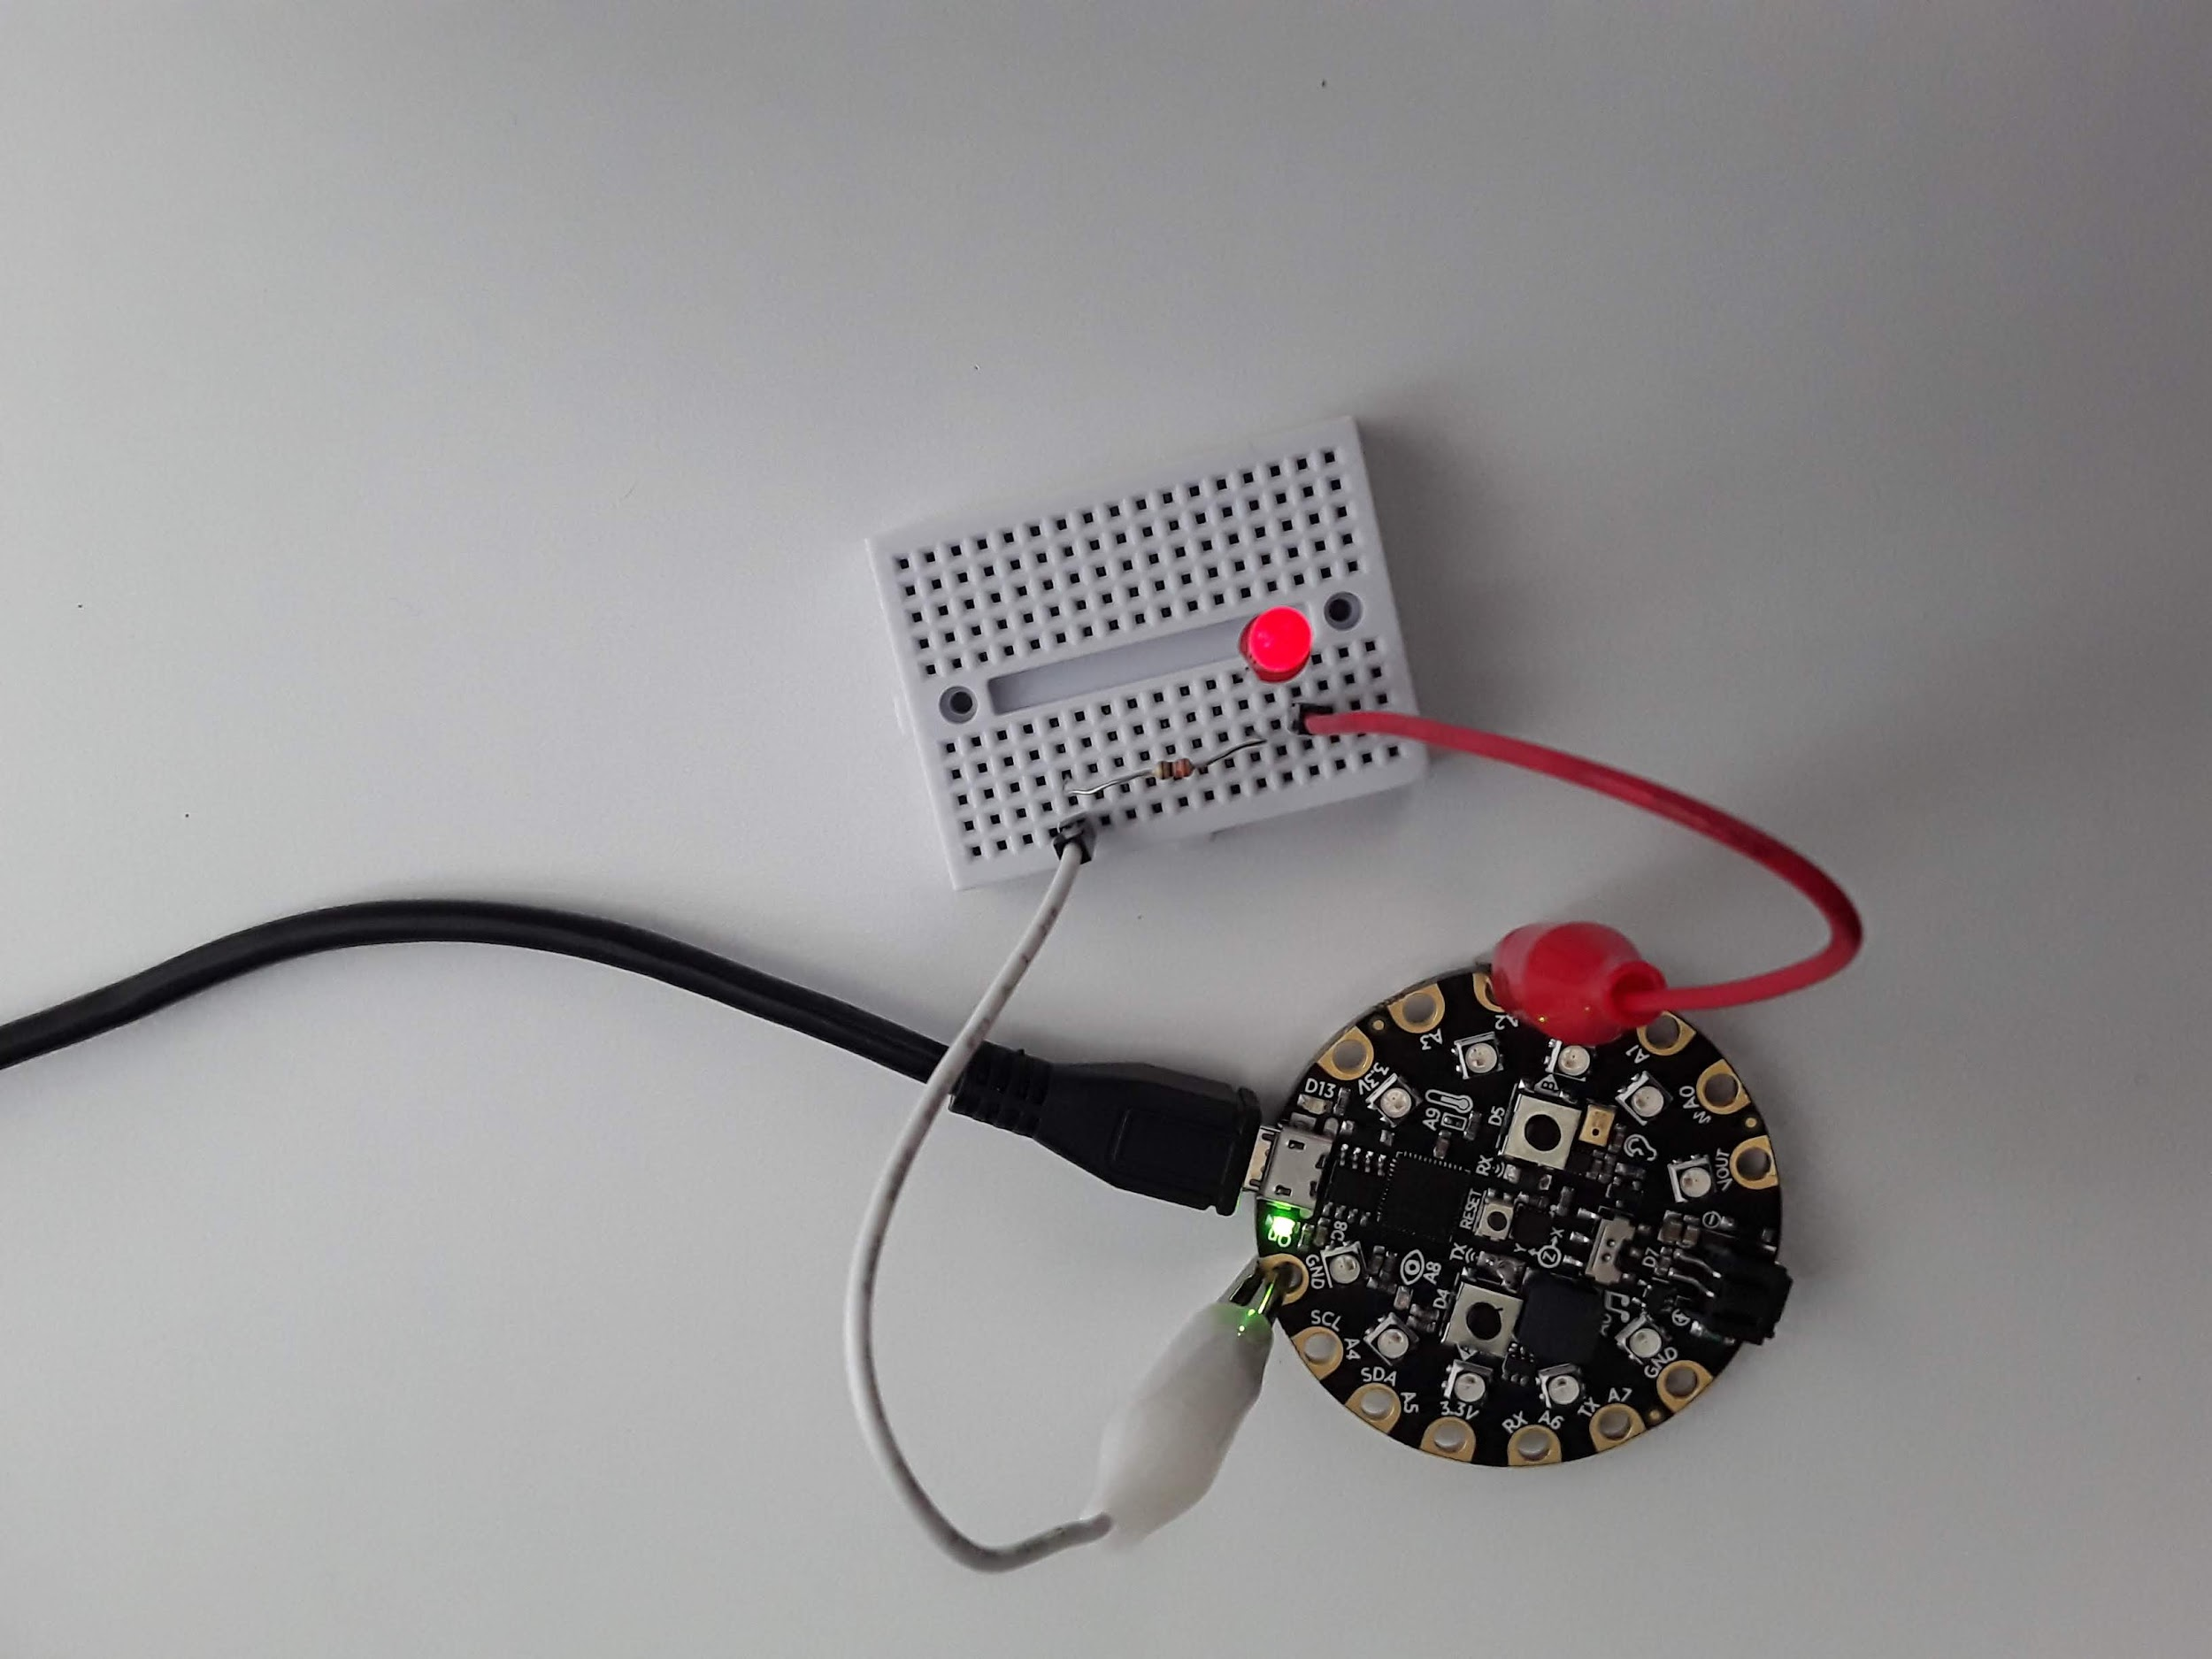
\includegraphics[width=\textwidth]{Figures/LED4.jpeg}
  \end{center}
\end{figure}

\subsection{LED with CPX button}

Finally, I want to use one of the buttons on the CPX to blink the LED
hooked up to pin A2. For this code to work you first need to detect a
button press and then tell the program to change the light from True
to False depending on what it’s current status is. This one is a bit
more difficult so I’ll include the code here and discuss the code
itself. Here is my circuit (identical) to the previous one with Button
A on the CPX pressed down. 
\begin{figure}[H]
  \begin{center}
    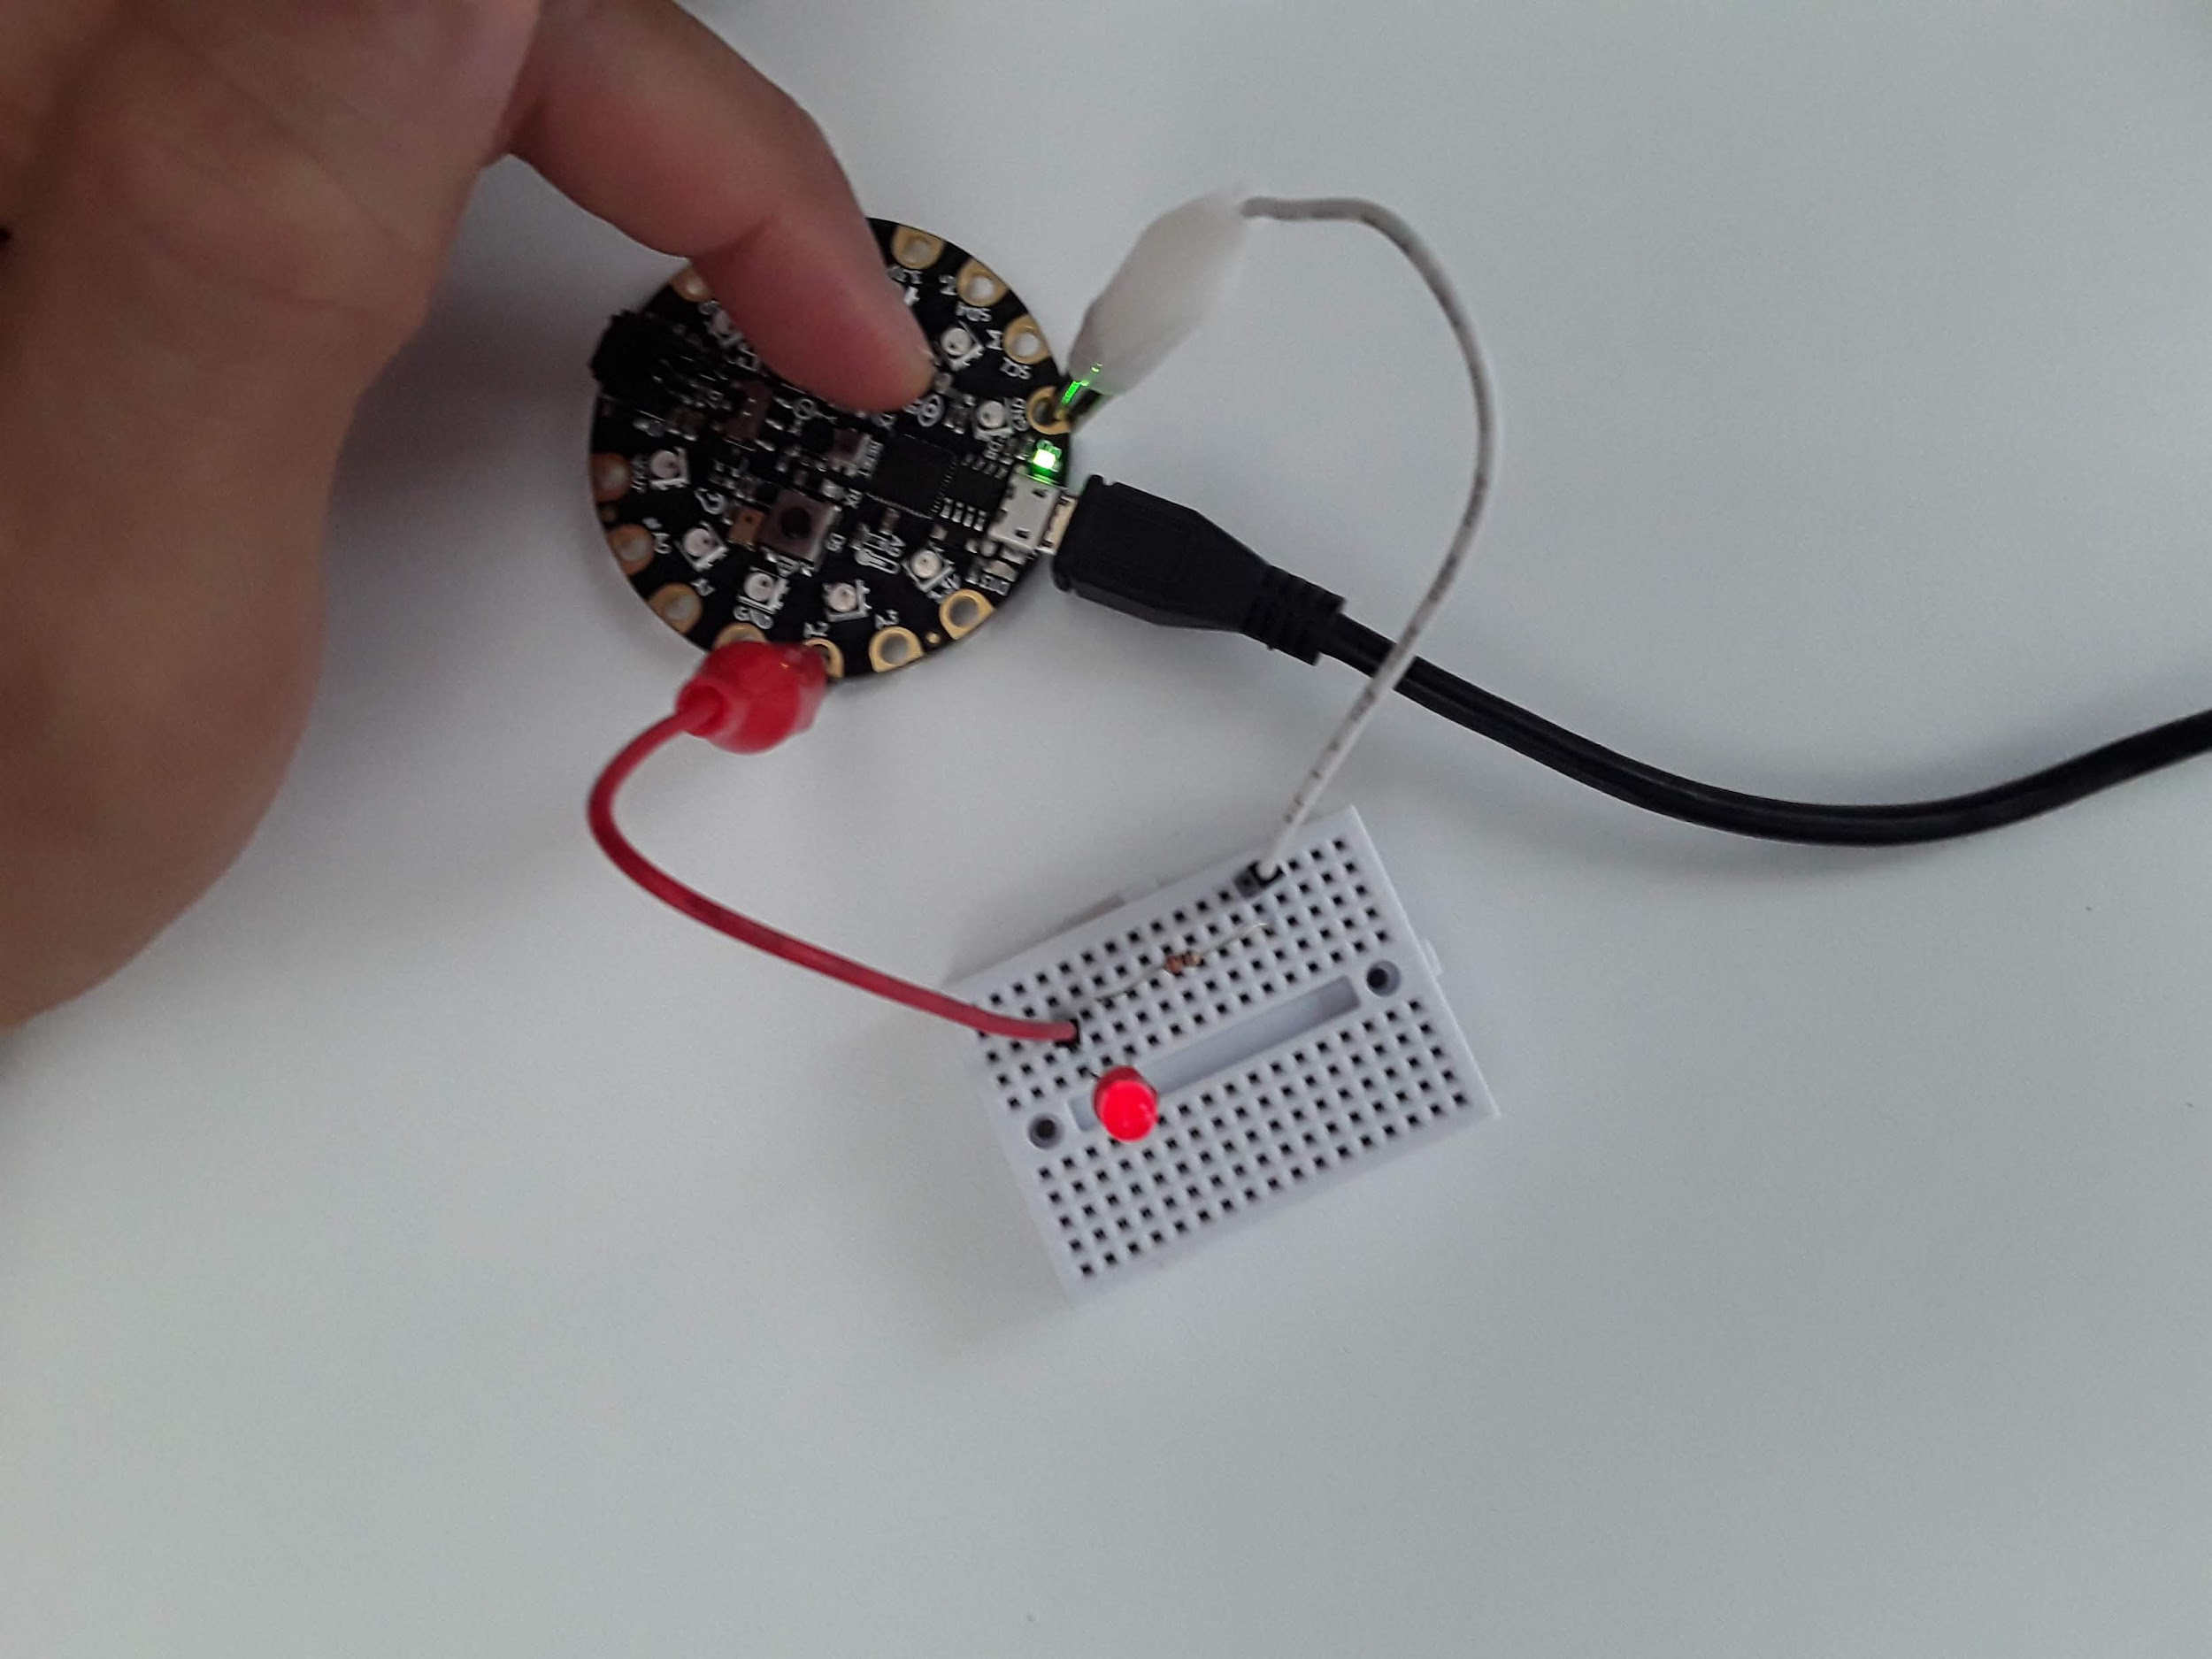
\includegraphics[width=\textwidth]{Figures/LED5.jpeg}
  \end{center}
\end{figure}
Alright so how do we detect a button press? Well the documentation on
this is not so straight forward. What we want to do is detect the
INPUT of a digital signal and then do something if we detect that
signal. Here’s the code I created to get it to work.
\begin{figure}[H]
  \begin{center}
    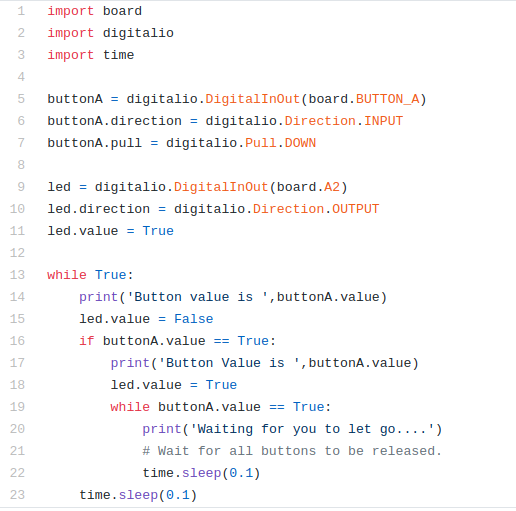
\includegraphics[width=\textwidth]{Figures/button_blink.png}
  \end{center}
\end{figure}
The code above is an image. You could type exactly what you see and
hope you don't type any errors (which is highly unlikely) or you could
look for my code on my
\href{https://github.com/cmontalvo251/Microcontrollers/tree/master/Circuit_Playground/CircuitPython}{Github}. Have
you bookmarked this link yet? I recommend you do so!!! So you're
making a code about Buttons....hmmm. Click that Github link. Where do
you think the code about Buttons is located? Anywho, let's talk about
the code.

The first 3 lines are exactly the same as before. Line 5 through 7 are
similar to creating the “led” variable except we’re using {\it BUTTON\_A} as
the board value and setting the direction to {\it INPUT}. Finally we’re
setting the pull direction to {\it DOWN}. This means the button acts like a
pull down resistor and when it’s pressed the value of the button goes
{\it HIGH}.

Lines 9-11 are the same as before. We create an led variable and tell
the CPX that the led is hooked up to pin A2. We then start the while
loop on line 13. First if you click the Serial button you’ll see the
text ‘Button value is False’. It’s False because {\it buttonA.value} is not
being pressed. On line 15 the led is set to False (turned off). On
line 16 the button value is checked using an if statement as to
whether or not the button is pressed (True). If the button is pressed,
the user will be notified that the button is pressed on line 17 and
the led will be set to True (on) in line 18. Lines 19-22 are while
loop that will notify the Serial monitor that you must let go of the
button before the code can continue to the main while loop. The
{\it time.sleep} functions are there to make sure a human can operate the
button without code running faster than a human can press a
button. When I press the button down here is the output I get from the
{\it Serial} monitor. 
\begin{figure}[H]
  \begin{center}
    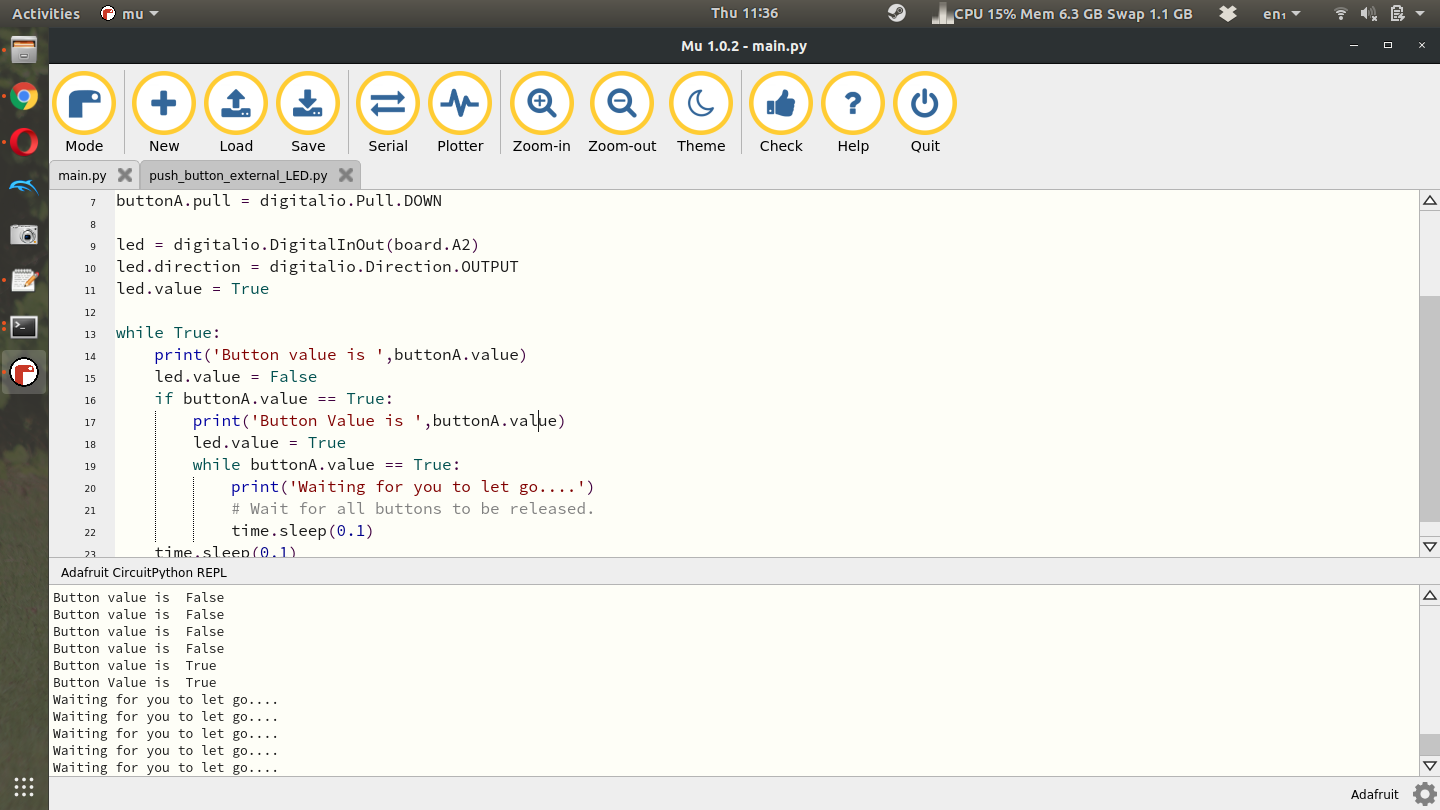
\includegraphics[width=\textwidth]{Figures/MuButton.png}
  \end{center}
\end{figure}
Here you’ll see 4 lines that say ``Button value is False" and then two
lines that say ``Button value is True" followed by 5 lines that say
``Waiting for you to let go...". See if you can get this code to work and
play with it and modify it as you see fit. By the way, the LED
connected to pin D13 has this exact same circuitry, an LED a resistor,
it’s all just soldered to the PCB so you don’t have to build it using
a breadboard. Hopefully now you have some appreciation for buttons and
LEDs!! 

\subsection{Assignment}

Once you've done the exercise above, upload a PDF with all of the
photos and text below included. My recommendation is for you to create
a Word document and insert all the photos and text into the
document. Then export the Word document to a PDF. For videos I suggest
uploading the videos to Google Drive, turn on link sharing and include
a link in your PDF.  

\begin{enumerate}[itemsep=-5pt]
\item Include a photo of your circuit with your LED turned on using VOUT (make sure your face is in the photo) - 20\%
\item Include a photo of your circuit with your LED turned on using 3.3V (make sure your face is in the photo) - 20\%
\item Include a video of you turning your LED on and off with the push button (again make sure your face is in the video for enough time to say who you are and say hello) - 20\%
\item Include a video of your LED blinking on and off automatically by modifying the blink code (make sure your face is in the video for enough time to say who you are and say hello) - 20\%
\item Include a video of your LED blinking by pressing a button on the CPX (make sure your face is in the video for enough time to say who you are and say hello) - 20\%
\end{enumerate}
